%%%%%%%%%%%%%%%%%%%%%%%%%%%%%%%%%%%%%%%%%%%%%%%%%%%%%%%%%%%%%%%%%%%
% Method
% Team:
% Union
% Members: 
% Bernie Huang, Jim Lan, Hoang Tan, Kenny Hsu, Rahul Aditya, Tan Phat, Wei
% Relative files:
% Method_Union.tex
% Note:    
% Do not compile this file compile Main.tex to get the pdf file instead.
%%%%%%%%%%%%%%%%%%%%%%%%%%%%%%%%%%%%%%%%%%%%%%%%%%%%%%%%%%%%%%%%%%%
\section*{Method}
As mentioned in the background, our group use natural language processing in order to generate metadata. 
The scope of metatada processing is about producing at least three types of metadata include author name, title and abstract. 
This is the least we want to produce within the time frame of this course. 
Once accomplishing the 3 types of metadata, we will extend the scope of our project, intimidate the scheme to produce other remaining metadata such as doix number, journal name, volume number and so on. 
If time is still on our side, we will even extend the scope our project further and join other teams to produce a search engine. 
Following discussion are our plan to complete extracting the 3 first types of metatata from PDF files.
\subsection*{Title extraction}
We chose python to be the program to catch the title and other metadata as well. First step, we import some necessary packages and functions as following:
\begin{enumerate}
	\item re: Regular expression package
	\item os: This function can connect the python to operating system, so that we can call the path
	\item nltk: A natural language toolkit. We use the corpus plaintext function to build the txt file in a folder as corpus.
	\item string:The string package includes a lot of classes such as lowercase, uppercase,punctuation,digits or whitespace...etc. 
\end{enumerate}  
To begin, we convert all PDF files we want to deal with into a txt file and set the path and store them in specific folder. 
Then, regular expression in python can help capturing the first sentence in the txt files, which have been converted and stored in specific folder in previous step. 
Afterward, we intend to produce the title of the article in a txt file.   

\subsubsection*{Author extraction}


\subsubsection*{Abstract extraction}
	Developing from previous theory mentioned in the background section, we use the python to catch the abstract. The following step is below
	%\begin{center}
	%	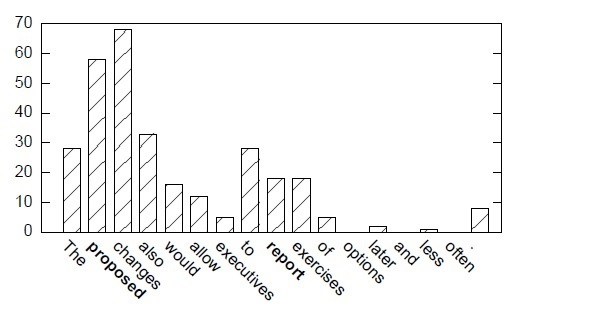
\includegraphics[width=\columnwidth]{Union_Background_Chart_2}
	%\end{center}
	The pdf is converted into txt file.Thus, it will create the txt file. The work is done by hand coding. For detailed coding scheme, we have presented it in the appendix at the end of this report\\ 
	After being able to read the txt file on every line, the python will detect the content of the abstract. In order to do so, we strip the text between "abstract" label and "introduction" label.\\ 	
	abstract-database:including the condition\\
	1. capital         "ABSTRACT"\\
	2. lower case      "abstract"\\
	3. in the sentence "Abstract—Word sense ....."\\
	4. and so on \\
	In the process building "abstract database", we are aware of different papers may have different form of structures and writing style, we search through numbers of articles from different journals. Number of article found is 100, from 20 different journals including The Lancet, Progress in Energy and Combustion Science, Chemical Analysis and so. Search results for sections such as Theoretical, Methods, Results, Discussion, Conclusion, Acknowledgements are also obtained.  Table below are the results of the search.\\
	\begin{center}
		%\includegraphics[width=\columnwidth]{Table for method Union}.\\
		%\includegraphics[width=\columnwidth]{Table 2 for method Union}.\\
		%\caption{Result of finding all forms of "abstract", "introduction" written by different authors}
	\end{center}
	Then our program will read the txt file on every line.If the python detects the abstract-database-stop's words ,it will stop to catch the sentences.\\ 
	abstract-database-stop:including the following conditions
	1. the blank line
	2. specific words in the beginning "Keywords"
	3. and so on.\\
	The intended output are sentences extracted to the txt file. To further validate if the program can run precisely, members randomly search for articles (10 articles) to test the programs. The program was run successfully and all abstracts was extracted from the text. \\ 	
	

\subsubsection*{Search sentences}
\begin{itemize}
	\item I use python to complete the task. 
	\begin{center}
		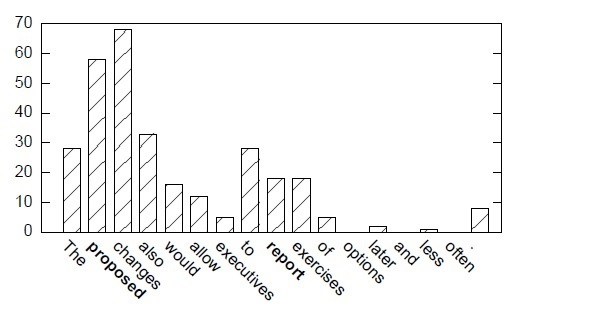
\includegraphics[width=0.8\columnwidth]{Union_Background_Chart_2}
	\end{center}
	\item First,turn the PDF to the txt file .(Make the programe easy to read file)\\ 
	\item Second,read the txt file by lines.\\ 	
	\item Third,create the array to divide the section of the articles.\\ 	
	\item Forth,expend the array to divide the section clearly.\\ 	
	\item Fifth,Users search the sentence.The programe search all sections by this sentence.\\
	\item Sixth,Show the results\\  		
	
\end{itemize}
Our project has four remaining weeks to complete (counting from 26 May 2016). 
So we use scrum management to speed up our process.


\subsubsection*{Factuality}

In the process of producing metadata, which are should be the most precise information and representing the text, validity of such metadata must be checked. 
Therefore tools for fact checks are developed based on linguistic techniques. 
The tool could detect facts and excludes authors' subjective opinions \cite{Agerri2014}. 
From the authors's perspective, the two main set of tools having such functions is TIMEBANK and FACTBANK.(yes, the authors used capitalized name)

TIMEBANK was first proposed in \cite{pustejovsky2003timebank}. 
The idea was based on that English language has different tenses which could be exploited as signals for fact check. 
An example as below could help to clarify the ideas. Let's examine these sentence:

\begin{itemize}
	\item I will go to Chimei museum tomorrow.
	\item Chimei museum is near Tainan District.
	\item I was in UK in 2012.
\end{itemize}

The first sentence is simple future tense which imply something has never actually happened, the second sentence is simple present tense which can directly imply facts, and the last sentence is in simple past tense which is about something already happened (which is facts), but is no longer a fact right now, so such fact must be used with caution. 

The reason for introducing such tool is that even scientific research articles can be glittering with subjective comments, opinions or even assumption from authors \cite{schultze2000confessional}. In addition to TIMEBANK, many other tools can be another filter for fact extraction. 
\cite{Dave2003mining} identify words, clauses and phrases that show emotional state of the authors. 
The choice in expression of facts could also be a helpful indicator to show whether authors are subjectively supporting a cause, an opinion and so on \cite{Wiebe2005}. 
Among these mentioned approaches, this paper highly favors creation a kind of thesaurus compiled of linguistic signaling for non-factually statements such as FACTBANK, which is built by \cite{Sauri2009}. 
Following example shows how subjective statements can be picked out.

\begin{itemize}
	\item Channelization would guarantee high flow velocity in rivers, flooding and consequent degradation of riparian community (1a)
	\item Funding agencies would be happy with big entrepreneurs, instead of small and medium enterprises (1b)
	\item Tolerance to dictatorship would has negative influences on anarchist movement (2a)
	\item Tolerance to dictatorship would doom anarchist movement (2b)
\end{itemize}

It is easy to find in statement (1a) is an absolute fact. 
Statement (1b) is however affected by emotional state of authors. 
After re-writing (1b) into: Funding agencies lend more money with lower interest rate to big entrepreneurs, instead of small and medium enterprises, sentence (1b) become a face-based statement. 
In another case, statement (2a) is a fact-based statement while in statement (2b), authors are stressing their dislike toward dictatorship.

Fact checks in language generation is a new field but many useful tools have been developed. 
Each of them has their own function and could complement each others. 
In the limit of this study, we are using both of TIMEBANK and FACTBANK together for fact check.



\subsubsection*{Language generation}

Natural language generation (NLG) is one branch of natural language processing. 
The goal is generating the words human being using via machine automatically. 
To use this technique, six basic activities are done: 
\begin{enumerate}
	\item content determination: In this active, we create some messages which are communicated in the text. 
	These messages shall be labeled and the entity in the messeges is also distinguished, which is convenient for us to use these data to the following step.
	\item discourse planning: This part is closely related to the previous part. 
	We determin the order and the structure of the messeges.
	\item sentence aggregation:This part combin several messeges in to sentence. 
	Although some of messeges have been a sentence, we can improve the influency of messeges by combining them.
	\item lexicalization: This part make the messege more precise by use the specific words and concepts. 
	Then people can get the idea of the messeges more quickly.
	\item referring expression generation: This part is a litte same as the previous part. 
	But the difference is that this part differentiate the one domain to the other domains.
	\item linguistic realization: Last part is to make the expression follow the rules of grammer, part of speech and the natural language rule.
\end{enumerate}
\cite{aramossoto2016onthe}.\todo{Where? Please explain the 6 terms. What are they?} The advantage of this technique is that it is flexible, since there is no standardization. 
But it also has the difficulty in the implication of this technique.\cite{aramossoto2016onthe}No standardization means that no rules can be followed. Without logic method, It is almost impossible to code and realized by computer.
Thus, the another concept is proposed. This way has the logical method, also the algorithm is easy to realize.
The technique is linguistic discription of data.\todo{Now you jump too far. More explanations are needed.}
Linguistic description of data (LDD) is a concept that applied the fuzzy set theory in the linguistic field. At the beginning, comparing to the NLG field, it is a newer technique to solve the problem of language generation. 
However, the basic steps of LDD have been built. 
The four main parts in this technique are input data, linguistic variable, fuzzy quantifiers and evaluation criteria \cite{aramossoto2016onthe}. Some of them are similar to the concept. 
The advantage of this technique is that it has been implied in many fields like weather forecast \cite{Ramos-SotoBBT14}. Also, many practical methods have been proposed. However, it still has a long way to go.

These two techniques are usually combined together nowadays. The concept of NLG and the practical approach of LDD could be used in the same time to provide the better performance in language generate field.
\newpage % Ends the current page and causes all figures and tables to be printed